\documentclass{article}
\usepackage{tikz}
\renewcommand*\familydefault{\sfdefault}
\usepackage[american]{circuitikz}

\begin{document}
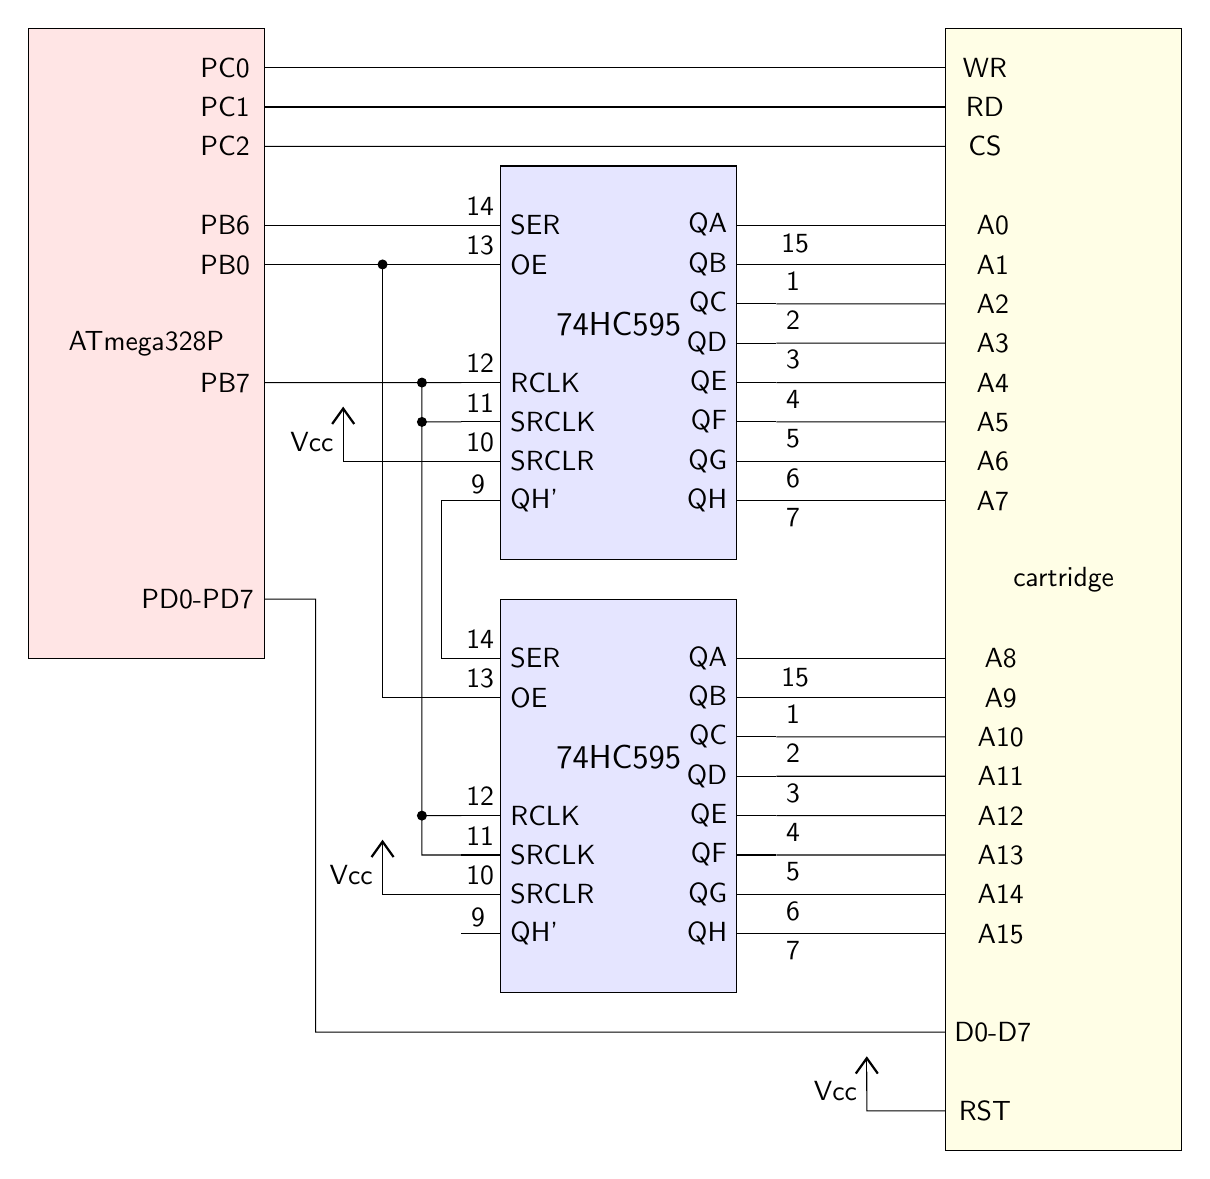
\begin{tikzpicture}
% Variables: 1 := position, 2 := ID.
\def\74xx595(#1)#2{
    \begin{scope}[shift={(#1)}]
        \draw[fill=blue!10] (-1.5, -2.5) rectangle (1.5, 2.5);
        \draw (0,0.5) node [align=center]{\large 74HC595};
        \draw (-1.5,1.75) node [right]{SER} -- +(-0.5,0) node [anchor=-135]{14} coordinate (#2 SER);
        \draw (-1.5,1.25) node [right]{OE} -- +(-0.5,0) node [anchor=-135]{13} coordinate (#2 OE);
        \draw (-1.5,-0.25) node [right]{RCLK} -- +(-0.5,0) node [anchor=-135]{12} coordinate (#2 RCLK);
        \draw (-1.5,-0.75) node [right]{SRCLK} -- +(-0.5,0) node [anchor=-135]{11} coordinate (#2 SRCLK);
        \draw (-1.5,-1.25) node [right]{SRCLR} -- +(-0.5,0) node [anchor=-135]{10} coordinate (#2 SRCLR);
        \draw (-1.5,-1.75) node [right]{QH'} -- +(-0.5,0) node [anchor=-135]{9} coordinate (#2 QH');
        \draw (1.5,1.75) node [left]{QA} -- +(0.5,0) node [anchor=135]{15} coordinate (#2 QA);
        \draw (1.5,1.25) node [left]{QB} -- +(0.5,0) node [anchor=135]{1} coordinate (#2 QB);
        \draw (1.5,0.75) node [left]{QC} -- +(0.5,0) node [anchor=135]{2} coordinate (#2 QC);
        \draw (1.5,0.25) node [left]{QD} -- +(0.5,0) node [anchor=135]{3} coordinate (#2 QD);
        \draw (1.5,-0.25) node [left]{QE} -- +(0.5,0) node [anchor=135]{4} coordinate (#2 QE);
        \draw (1.5,-0.75) node [left]{QF} -- +(0.5,0) node [anchor=135]{5} coordinate (#2 QF);
        \draw (1.5,-1.25) node [left]{QG} -- +(0.5,0) node [anchor=135]{6} coordinate (#2 QG);
        \draw (1.5,-1.75) node [left]{QH} -- +(0.5,0) node [anchor=135]{7} coordinate (#2 QH);
    \end{scope}
}
\74xx595(0,0){1}
\74xx595(0,-5.5){2}
\draw(1 QH')
    to [short] ++(-0.25,0)
    to [short] ($ (2 SER) - (0.25,0) $)
    to [short] (2 SER);
\draw(1 RCLK)
    to [short, -*] ++(-0.5,0) coordinate (CLK)
    to [short, -*]($ (1 SRCLK) - (0.5,0) $) coordinate (TEMP)
    to [short] (1 SRCLK)
    to [short] (TEMP)
    to [short, -*] ($ (2 RCLK) - (0.5,0) $) coordinate (TEMP)
    to [short] (2 RCLK)
    to [short] (TEMP)
    to [short] ($ (2 SRCLK) - (0.5,0) $)
    to [short] (2 SRCLK);
\draw(1 OE)
    to [short, -*] ++(-1.0,0) coordinate (OE)
    to [short] ($ (2 OE) - (1.0,0) $)
    to [short] (2 OE);
\draw(1 SRCLR)
    to [short] ++(-1.50,0)
    to node[vcc,label=left:Vcc]{} ++(0,0.5);
\draw(2 SRCLR)
    to [short] ++(-1.0,0)
    to node[vcc,label=left:Vcc]{} ++(0,0.5);
\draw(CLK)
    to [short] ++(-2.0,0) coordinate (CLK);
\draw(1 SER)
    to [short] ++(-2.5,0) coordinate (SER);
\draw(OE)
    to [short] ++(-1.5,0) coordinate (OE);
\draw[fill=red!10]($ (1 SER) + (-5.5,2.5) $) coordinate (ATMEGA1) rectangle ++(3.0, -8.0) coordinate (ATMEGA2);
\draw($ (ATMEGA1) + (3,-0.5) $) coordinate (PC0)
    to [short] ++(0.65,0)
    to [short] ++(8,0) coordinate (WR);
\draw($ (ATMEGA1) + (3,-1) $) coordinate (PC1)
    to [short] ++(0.65,0)
    to [short] (WR |- PC1) coordinate (RD);
\draw($ (ATMEGA1) + (3,-1.5) $) coordinate (PC2)
    to [short] ++(0.65,0)
    to [short] (WR |- PC2) coordinate (CS);
\draw($ (ATMEGA2) + (0,0.75) $) coordinate (PORTD)
    to [short] ++(0.65,0)
    to [short] ++(0,-5.5)
    to [short] ++(8,0) coordinate (D0-D7);
\draw[fill=yellow!10]($ (WR) + (0,0.5) $) coordinate (CART1) rectangle ($ (D0-D7) + (3.0,-1.5) $) coordinate (CART2);
\draw(1 QA) to [short] (CART1 |- 1 QA) coordinate (A0);
\draw(1 QB) to [short] (CART1 |- 1 QB) coordinate (A1);
\draw(1 QC) to [short] (CART1 |- 1 QC) coordinate (A2);
\draw(1 QD) to [short] (CART1 |- 1 QD) coordinate (A3);
\draw(1 QE) to [short] (CART1 |- 1 QE) coordinate (A4);
\draw(1 QF) to [short] (CART1 |- 1 QF) coordinate (A5);
\draw(1 QG) to [short] (CART1 |- 1 QG) coordinate (A6);
\draw(1 QH) to [short] (CART1 |- 1 QH) coordinate (A7);
\draw(2 QA) to [short] (CART1 |- 2 QA) coordinate (A8);
\draw(2 QB) to [short] (CART1 |- 2 QB) coordinate (A9);
\draw(2 QC) to [short] (CART1 |- 2 QC) coordinate (A10);
\draw(2 QD) to [short] (CART1 |- 2 QD) coordinate (A11);
\draw(2 QE) to [short] (CART1 |- 2 QE) coordinate (A12);
\draw(2 QF) to [short] (CART1 |- 2 QF) coordinate (A13);
\draw(2 QG) to [short] (CART1 |- 2 QG) coordinate (A14);
\draw(2 QH) to [short] (CART1 |- 2 QH) coordinate (A15);
\draw($ (CART1 |- CART2) + (0,0.5) $)
    to [short] ++(-1.0,0)
    to node[vcc,label=left:Vcc]{} ++(0,0.5);

\node[] at ($ (SER) - (0.5,0) $) {PB6};
\node[] at ($ (CLK) - (0.5,0) $) {PB7};
\node[] at ($ (OE) - (0.5,0) $) {PB0};
\node[] at ($ (PORTD) - (0.85,0) $) {PD0-PD7};
\node[] at ($ (PC0) - (0.5,0) $) {PC0};
\node[] at ($ (PC1) - (0.5,0) $) {PC1};
\node[] at ($ (PC2) - (0.5,0) $) {PC2};
\node[] at ($ (WR) + (0.5,0) $) {WR};
\node[] at ($ (RD) + (0.5,0) $) {RD};
\node[] at ($ (CS) + (0.5,0) $) {CS};
\node[] at ($ (A0) + (0.6,0) $) {A0};
\node[] at ($ (A1) + (0.6,0) $) {A1};
\node[] at ($ (A2) + (0.6,0) $) {A2};
\node[] at ($ (A3) + (0.6,0) $) {A3};
\node[] at ($ (A4) + (0.6,0) $) {A4};
\node[] at ($ (A5) + (0.6,0) $) {A5};
\node[] at ($ (A6) + (0.6,0) $) {A6};
\node[] at ($ (A7) + (0.6,0) $) {A7};
\node[] at ($ (A8) + (0.7,0) $) {A8};
\node[] at ($ (A9) + (0.7,0) $) {A9};
\node[] at ($ (A10) + (0.7,0) $) {A10};
\node[] at ($ (A11) + (0.7,0) $) {A11};
\node[] at ($ (A12) + (0.7,0) $) {A12};
\node[] at ($ (A13) + (0.7,0) $) {A13};
\node[] at ($ (A14) + (0.7,0) $) {A14};
\node[] at ($ (A15) + (0.7,0) $) {A15};
\node[] at ($ (D0-D7) + (0.6,0) $) {D0-D7};
\node[] at ($ (CART1 |- CART2) + (0.5,0.5) $) {RST};
\node[] at ($ (ATMEGA1) + (1.5,-4.0) $) {ATmega328P};
\node[] at ($ (CART1) + (1.5,-7.0) $) {cartridge};
%\node[rotate=90,font=\fontsize{24pt}{24pt}\selectfont] at ($ (1 QB) + (0.75,-1.5) $) {...};
%\node[rotate=90,font=\fontsize{24pt}{24pt}\selectfont] at ($ (2 QB) + (0.75,-1.5) $) {...};
\end{tikzpicture}
\end{document}
